\documentclass[]{article}  % Comment this line out

%\IEEEoverridecommandlockouts                              % This command is only
                                                          % needed if you want to
                                                          % use the \thanks command
%\overrideIEEEmargins

\usepackage[margin=1in]{geometry}
\usepackage{amsmath}    % need for subequations
\usepackage{graphicx}   % need for figures
\usepackage[font=footnotesize,labelfont=footnotesize]{caption}
\usepackage{verbatim}   % useful for program listings
\usepackage{color}      % use if color is used in text
%\usepackage{begin{subfigure} % use for side-by-side figures
\usepackage{subcaption}
\usepackage{hyperref} % use for hypertext links, including those to external documents and URLs
\usepackage{multirow}
\usepackage{rotating}
\usepackage{array}
\usepackage{xspace}
\usepackage{indentfirst}
\usepackage{amssymb}
\usepackage{float}
\usepackage{algorithm}
\usepackage{algorithmic}
\usepackage{comment}
\usepackage{sidecap}
\usepackage{booktabs}

\title{A Visibility-Based Combinatorial Data Structure for
Mobile Robots in Polygons}

\author{Alexandra Q. Nilles, Yingying Ren, Steven M. LaValle% <-this % stops a space
%\thanks{This work was partially supported by National Science Foundation (award numbers CMMI-1100579 and IIS-1302393).}
}

\begin{document}


\maketitle

%%%%%%%%%%%%%%%%%%%%%%%%%%%%%%%%%%%%%%%%%%%%%%%%%%%%%%%%%%%%%%%%%%%%%%%%%%%%%%%%
%\begin{abstract}
%
%\end{abstract}

{\small
\begin{center}
\begin{quotation}
``Geometry is not true, it is advantageous." \\
\hfill    --- Henri Poincar\'e
\end{quotation}
\end{center}
}

%%%%%%%%%%%%%%%%%%%%%%%%%%%%%%%%%%%%%%%%%
\section{Introduction} 

This control strategy is largely chosen because of the ease of implementation.
It requires much less fine-grained proprioception than many other mobile robot
control algorithms, needing the robot to only have the ability to move forward
until reaching some obstacle, then the ability to rotate in place. We assume
from the beginning that there will be nondeterministic error in both of these
operations - especially when wheels are independently powered, robots rarely
move forward in truly straight lines, and rotation-in-place is similarly
difficult to achieve precisely. Both of these types of error are accounted for
by our nondeterministic state propagation. In fact, our approach does not assume
a fixed error distribution or range, but in fact produces the maximum allowable
error values constructively. Thus, this work lends itself well to the mobile
robot system design process - users can iteratively design environments and
robots such that the desired task has a strong guarantee of success.

The only type of error we do not
account for is ``sliding" along the environment boundaries, which may occur
during rotation or collision. However, many common commercial mobile robots
(such as vacuum robots) do not experience appreciable sliding.

% There has been rising interests in minimum sensing robots in recent years as swarm robots become more and more popular. 
In this paper, we consider simple robots with "bouncing" behaviors: robots which
travel in straight lines in the plane, until encountering an environment
boundary, at which point they rotate in place and set off again. A growing line
of work is considering the computational power of individual bouncing strategies
and their applications to robotic tasks and applications in biological contexts
\cite{ErLav13}, \cite{microorganism2017}, \cite{alam2017minimalist}.

We introduce a combinatorial, visibility-based data structure to organize and
compare these bouncing strategies in simple polygonal environments. The overall
idea is to discretize the environment boundary using visibility information,
creating equivalence classes (segments along the boundary) where the robot has a
similar set of choices from any point in the segment. We then construct a graph
representation of this environment where nodes are segments of the boundary, and
edges are transitions between segments (with associated control strategies). We
then extend previous results on the dynamics of composed transitions
\cite{NilBecLav17}, which give convenient guarantees on the stability of cycles
and contraction of robot state uncertainty. Finally, we demonstrate how to
formulate many common mobile robotic tasks as queries to this data structure.


\subsection{Robot Motion Model}\label{subsec:bounce_strategy}

A polygon is in general position if no $3$ vertices lie on the same line. For
the rest of this paper, we assume all polygons are in general position. All
index arithmetic is $\mod n$ throughout the paper.

A \emph{bouncing strategy} describes the robot's configuration change when it
encounters the boundary of a polygon. We will only consider the bounce occurred
inside an open edge of the polygon: the robot's behavior is undefined at a
vertex of the polygon.

A bouncing strategy defines a function space, where each function maps between 
points of the environment boundary, parameterized by the incoming trajectory
angle and optionally an angle $\theta$.

%Each bouncing strategy has a characterization function
%for $\vec{m}$ over parameters $\vec{n}$ and $\vec{l}$, where $\vec{n}$ is the
%unit vector for the normal of the bounce-off wall, $\vec{l}$ is the unit vector
%for the incoming direction, and $\vec{m}$ is the unit vector for the outgoing
%direction.
%
%\begin{itemize}
%    \item Specular Bounce (Billiard): $\vec{m} = f(\vec{l}, \vec{n})$, where \begin{eqnarray*}
%    f(\vec{l}, \vec{n}) = \vec{l} - 2(\vec{l}\cdot \vec{n})\vec{n}
%    \end{eqnarray*}
%    (``$\cdot$'' is the dot product operation between two vectors), which is equivalent to $(\vec{l}+\vec{m}) \cdot \vec{n} = 0$. This bouncing behavior is elastic and follows the most natural law: the incoming angle equals the outgoing angle \cite{geometry_billards}.
%    \item Fixed Angle Bounce: $\vec{m} = f(\vec{n}, \theta)$, where $\theta$ is a constant in $[-\frac{\pi}{2}, \frac{\pi}{2}]$, and \begin{eqnarray*}f(\vec{n}, \theta) = 
%    \begin{bmatrix} 
%    \cos(\theta) & \sin(\theta)\\
%    -\sin(\theta) & \cos(\theta)\\
%    \end{bmatrix}\vec{n}.\end{eqnarray*} In other words, the robot always bounces off the wall at a fix angle with respect to the normal.
%    \item Monotonic Fixed Angle Bounce: $\vec{m} = f(\vec{l}, \vec{n}, \theta)$, where $\theta$ is a constant in $(0, \frac{\pi}{2})$. Let $s = det(\begin{bmatrix} 
%    \vec{l}.x & \vec{l}.y\\
%    \vec{n}.x & \vec{n}.y\\
%    \end{bmatrix})$, and $\theta' = \frac{s}{|s|}\theta$ ($|s|$ denote the absolute value of $s$; the behavior for $|s| = 0$ is undefined). Then \begin{eqnarray*}f(\vec{l}, \vec{n}, \theta) = 
%    \begin{bmatrix} 
%    \cos(\theta') & \sin(\theta')\\
%    -\sin(\theta') & \cos(\theta')\\
%    \end{bmatrix}\vec{n}.\end{eqnarray*} This bouncing strategy is very similar to the Fixed Angle Bounce except for the monotonic restriction that the robot's incoming path and outgoing path have to be on the opposite sides of the normal.
%    
%    \item Relative Angle Bounce: $\vec{m} = f(\vec{l}, \beta)$, where $\beta$ is a constant in $[0, 2\pi)$, and \begin{eqnarray*}f(\vec{l}, \beta) = \begin{bmatrix}
%    \cos(\beta) & -\sin(\beta)\\
%    \sin(\beta) & \cos(\beta)\\
%    \end{bmatrix}\vec{l}.
%    \end{eqnarray*} The robot will rotate a fixed angle $\beta$ counter-clockwise when encountering the wall. It is possible that this rotation will cause the heading of the robot to still be facing into the wall, in which case this model usually has the robot perform the rotation again until it's heading points into the free space.
%\end{itemize}

% fixed vs. monotonic fixed vs. relative vs. specular

% parameterization for monotonic bounces: alpha + beta + gamma = pi

% all bounces are some function of incoming angle and wall normal

\subsection{Related Work}

In \cite{microorganism2017}, the authors show that a
\textit{Chlamydomonas reinhardtii} cell would bounce off a surface with a
monotonic fixed angle bounce. This line of work characterizes periodic and
chaotic trajectories in regular polygons, planar curves, and other environments.
They analyze dynamics of fixed bounce angles, without a focus on control.

\cite{LewOKa13} partially solved the navigation task with a very similar robot
model. Their robot moves in straight lines until encountering an environment
boundary, at which point it is able to rotate in place, with some nondeterministic but
bounded error. They then generate a strategy as a sequence of bounce angles which can navigate the robot between given start and end locations in a known environment. Their approach only allows "safe actions," which place
the entire forward projected state of the robot within a single
linear segment of the polygonal environment. They then solve the navigation task by
planning in a graph where each node is a point or segment
location of the robot, and edges are safe actions. However, this algorithm is
not complete, due to the restriction on safe actions -
sometimes the uncertainty of the actuators make it impossible to create a
strategy which only uses safe actions. Additionally, it requires hand-crafted
local planners for navigating long hallways, due to the way the environment
segmentation is done. At most, their graph search has $O(n^4)$ nodes, which is
the same complexity as our proposed data structure, but our method can also
achieve navigation without hand-crafted local planners due to the
visibility-based decomposition of the environment boundary.

In \cite{alam2017minimalist} and \cite{alam2018space}, the authors describe
navigation, coverage, and localization algorithms for a robot with a clock and
contact sensor that is capable of performing relative angle bounces. Their
approach uses a discretization of the robot configuration space and actuation
space, then searches the discretized dynamical system for limit cycles. The
algorithm is complete and correct up to discretization error - periodic
trajectories may exist which require bounce angles not allowed by the
discretization. Our work is very similar in spirit to this approach, however, we
use a more natural discretization induced by the environment geometry and
consider all possible bounce strategies in our combinatorial representation. Our
representation may be reduced to one which can be used to solve the same
problems as this work, by applying constraints on the types of bounces allowed.


\section{Combinatorial Visibility Data Structures}

We will provide an overview of some data structures related to visibility in
polygons, some of which we are using directly, and some of which provided
inspiration for this work.

\subsection{Visibility Graphs}


Let $P$ be a polygon in $\mathbb{R}^2$ with $n$ vertices
$(v_0, v_1, \ldots, v_{n-1})$. An edge of $P$ is represented as
$e_i = v_iv_{i+1}$.

The \textit{vertex visibility graph} $G_V(P) = (V, E)$ has $V = \{v_0, v_1, \ldots, v_{n-1}\}$ and $v_iv_j\in E$ if and only if the segment connecting $v_i$ and $v_j$ is completely contained in the interior of $P$. We call $v_i, v_j$ visible to each other if $v_iv_j\in E$. By definition, the vertex visibility graph for a convex polygon with $n$ vertices is a $n-$clique. Fig
\ref{fig:vvg} shows the visibility graph for a non-convex polygon.

\begin{figure}
    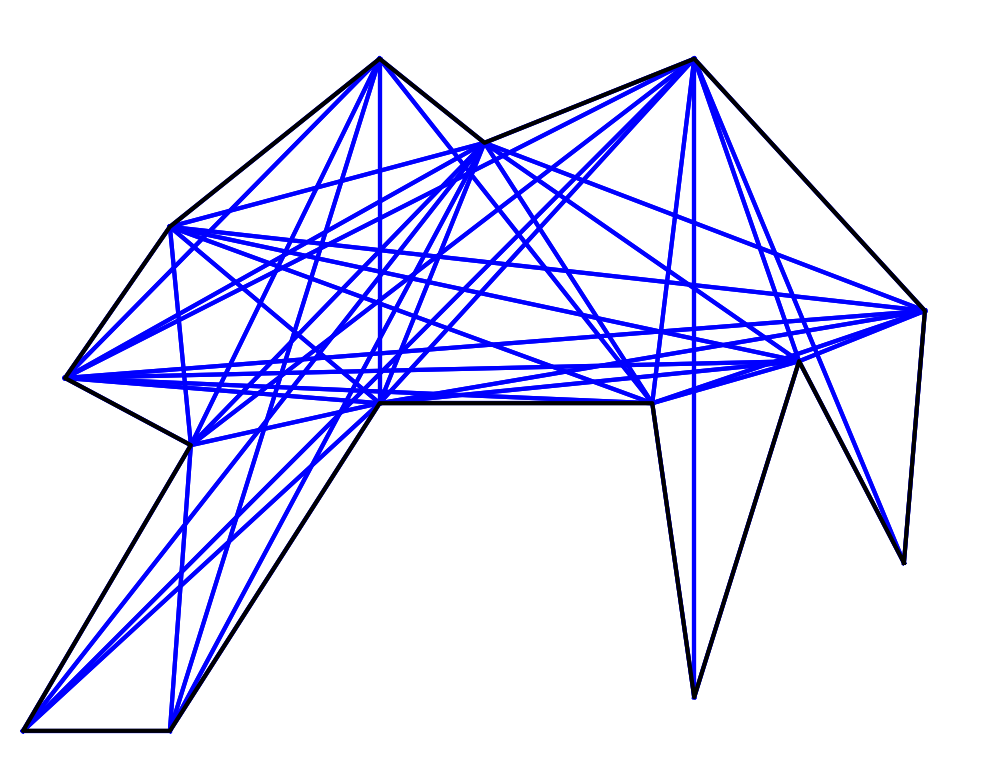
\includegraphics[width=0.8\linewidth]{figures/viz_graph.png}
    \centering
    \caption{The vertex visibility graph}\label{fig:vvg}
    \centering
\end{figure}

We can also define the \textit{vertex-edge visibility graph} for a polygon. Using the definition in \cite{rourke_viz}, the \textit{vertex-edge visibility graph} for $P$, $G_E(P) = (V, E)$, is a bipartite graph where $V = \{\text{all vertices and edges in $P$}\}$ and $v_ie_j\in E$ if and only if $v_i$ can see the interior of $e_j$, i.e., $\exists$ point $q$ on the open edge $e_j$ such that $v_i$ and $q$ are visible. \cite{rourke_viz} established that the vertex-edge visibility graph is equivalent to the edge-edge visibility graph.
Fig \ref{fig:veg} shows an example for vertex-edge visibility graph.

\begin{figure}
\centering
\begin{subfigure}{0.25\textwidth}
  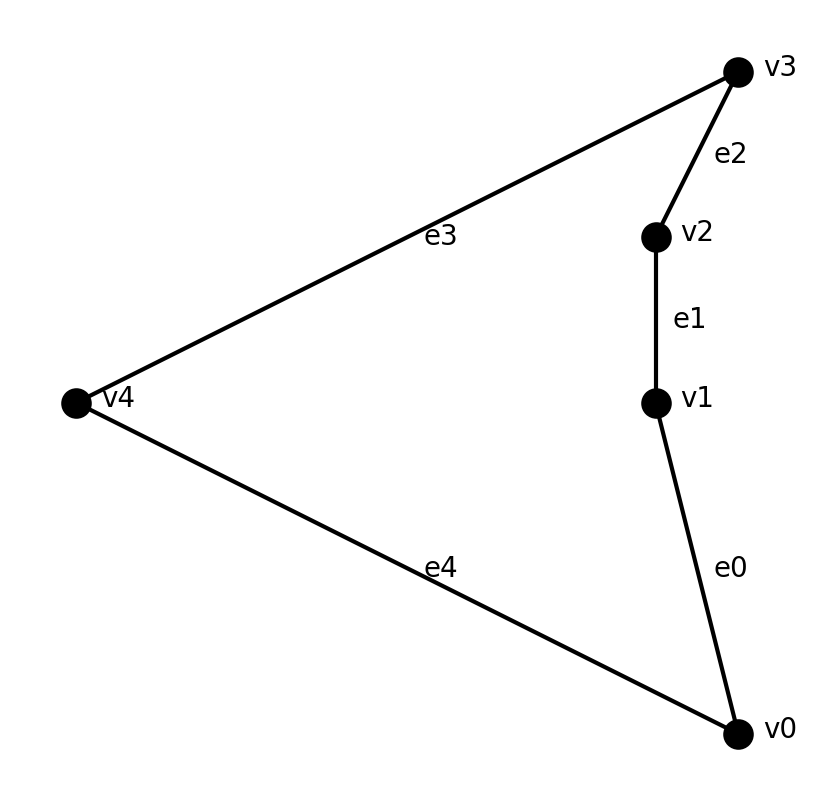
\includegraphics[width=0.6\linewidth]{figures/concave_pent.png}
  \label{fig:c_p}
\end{subfigure}%
\begin{subfigure}{0.25\textwidth}
  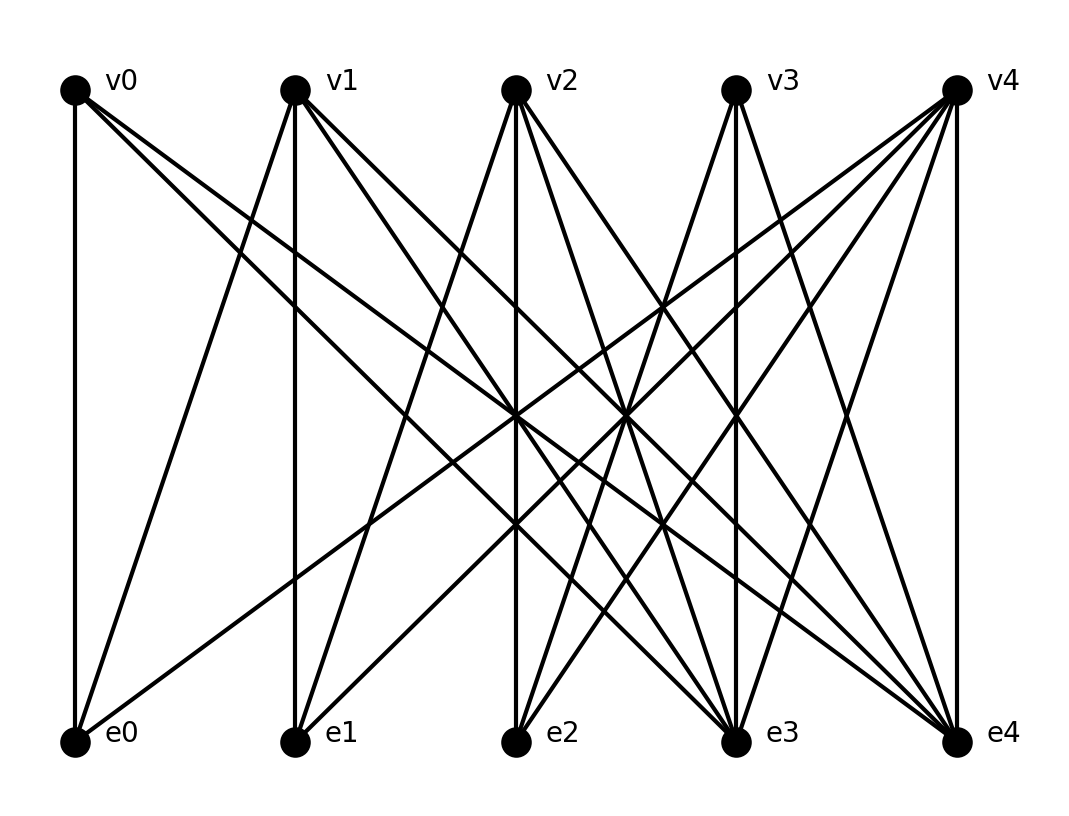
\includegraphics[width=0.8\linewidth]{figures/viz_edge_graph.png}
\end{subfigure}
\caption{A polygon and its corresponding vertex-edge visibility graph.\label{fig:veg}}

\end{figure}


\subsection{Partial local sequence}

The partial local sequence, defined in \cite{rourke_viz}, 
for a vertex $v_0$ in polygon $P$ is constructed 
by shooting a ray through $v_0$ from every vertex in $P$ that is visible from
$v_0$.

See Fig \ref{fig:pls} for an example of the vertices in the partial local
sequence of $v_0$ (blue dots with accompanying rays).

\begin{figure}[h]
    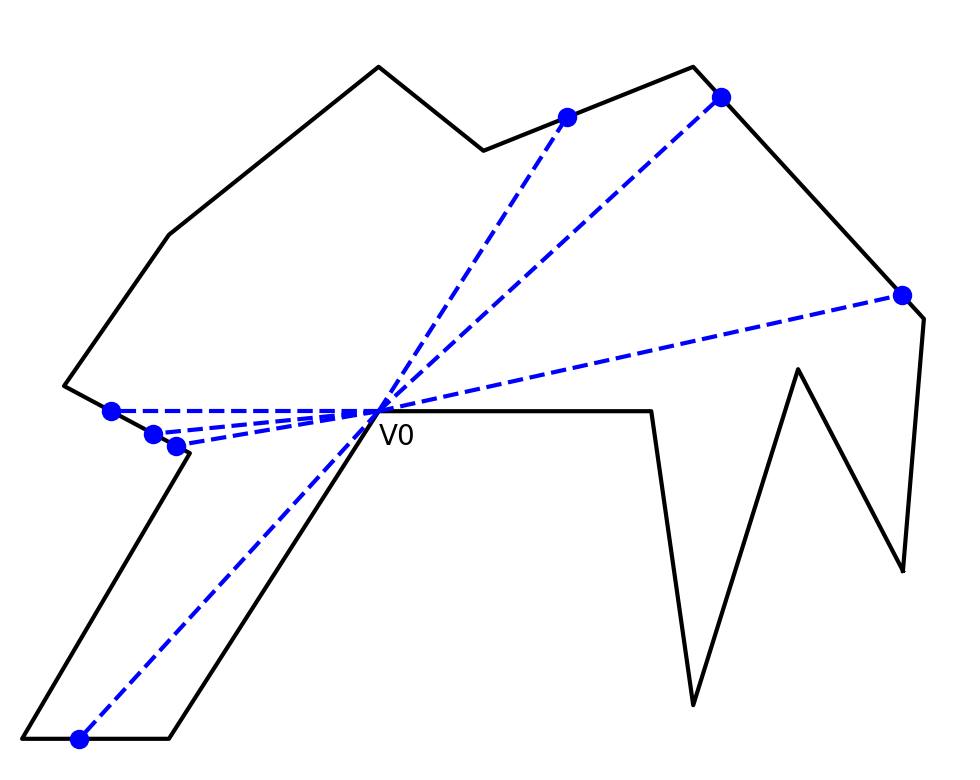
\includegraphics[width=0.8\linewidth]{figures/partial_local_sequence.png}
    \caption{Partial local sequence for $v_0$}\label{fig:pls}
    \centering
\end{figure}

The partial local sequences for vertices in a polygon is helpful for defining
the equivalence classes of edge visibility - each point in each partial local
sequence defines a \emph{transition event} where the visibility polygon of the
robot gains or loses edges if the robot were traversing along the boundary.


\subsection{Link diagram}

The link distance between two vertices in a polygon is the minimum number of line segments inside the polygon connecting the two vertices. The link distance between visible vertices is $1$. In Fig~\ref{fig:link_dis}, the link distance between $v_1$ and $v_2$ is 3.

The link diagram, as introduced in \cite{tan_sweep}, displays the link distance between any two points on the boundary of the polygon. The link diagram is our main motivation for creating a visibility diagram augmented with bouncing information.
\begin{figure}
    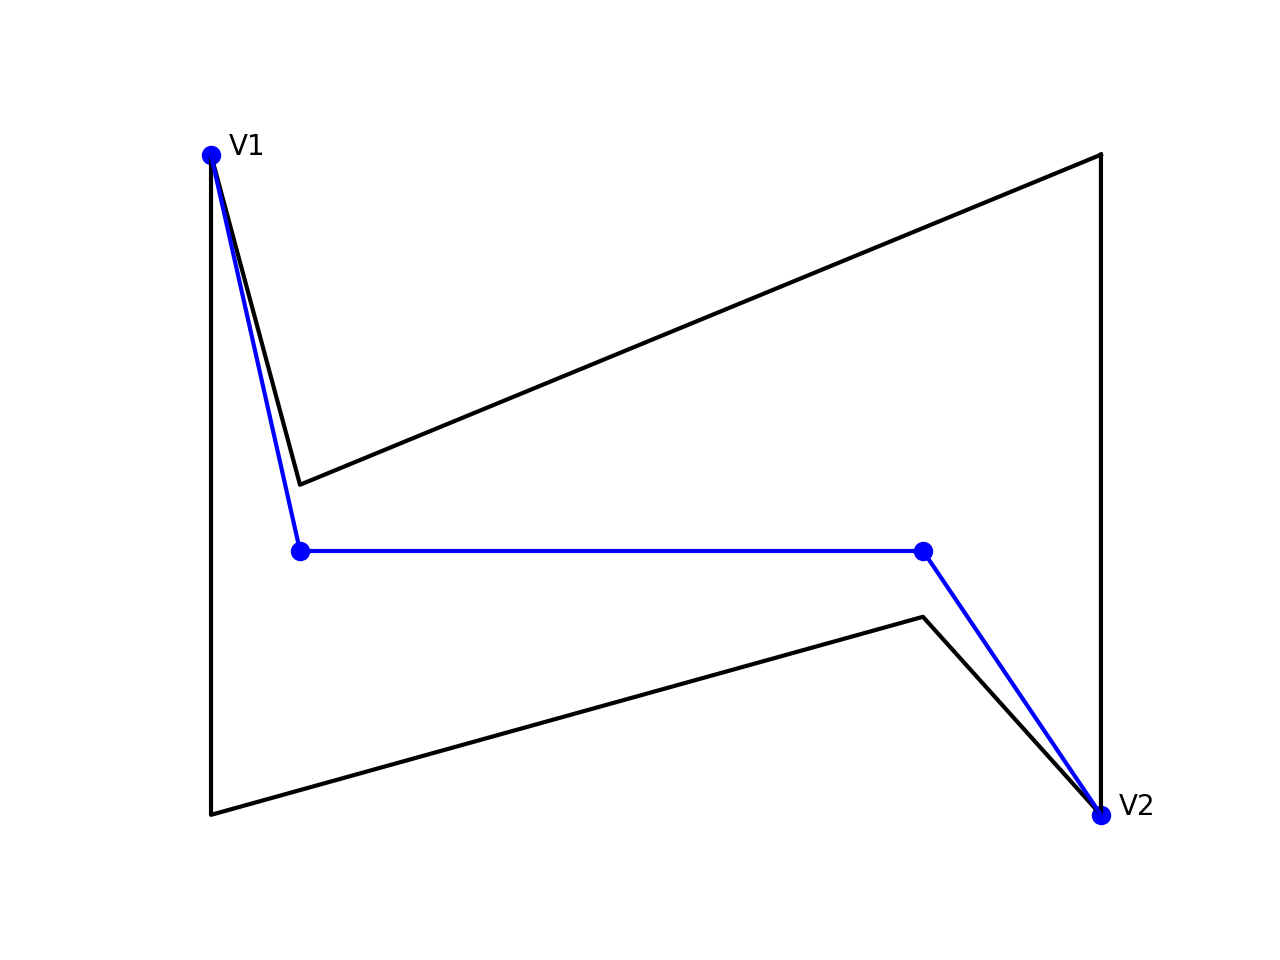
\includegraphics[width=0.6\linewidth]{figures/link_distance.png}
    \centering
    \caption{The link distance between $v_1$ and $v_2$ is 3, as shown by the three blue line segments connecting the two vertices.}\label{fig:link_dis}
    \centering
\end{figure}

\section{Bounce Visibility Diagram \label{bvd_def}}
We will now define the central structure for this paper, the
\textit{Bounce Visibility Diagram} for polygon $P$. We will first insert all new
vertices from the partial local sequence for all vertices into the
polygon $P$, creating the new polygon $P'$ with $m$ vertices. Each of these new
vertices marks a combinatorial change in the visibility polygon at the boundary
of the polygon as an agent traverses the boundary.

The $x-$axis of the diagram parameterizes the boundary of the new polygon,
denoted as $\partial P'$, in counterclockwise order as the interval $[0, m+1)$. The
enpoints of this interval are identified, though for visualization purposes we
do not represent this explicitly. We map every
point in $\partial P'$ to a point in $[0, m+1)$; vertex $v_i$ on $\partial P'$
will map to $x = i$; all points in the open edge $v_iv_{i+1}$ will uniformly map
to $(i, i+1)$. Let $f: [0, m+1)\mapsto \partial P'$ denote this
parameterization. We will generally use the variable $s$ to refer to points on
the boundary of $\partial P'$.

The vertical axis $\theta$ of the diagram has range $[0, \pi]$, representing all
the possible departure angles of the robot from point $s \in \partial P'$. 
At angle $0$, the robot is performing ``wall following": a bounce
to the next counterclockwise vertex.
Let the robot's ``forward direction'' be the direction of the edge that the
robot is on in counterclockwise order.

For each vertex $v_i$, we can define a function $B_i: [0, n) \mapsto [0, \pi]$
for the angle between the robot's forward direction and its direction to vertex
$v_i$ when the robot stands at $f(x)\in \partial P'$. $B_i$ are piecewise
continuous functions; the discontinuities occur when $x$ is an integer, or, in
other words, at the vertices of $\partial P'$. The original vertices in $P$ mark
discontinuities because the angle reference frame for the robot changes when it
moves to a new edge; the new vertices in $P'$ mark discontinuities because the
robot has different vertex visibility view around those vertices, which
motivates us to compute the partial local sequences in the first place.
Fig \ref{fig:bvd} shows an example of the bounce visibility diagram.

\begin{figure}

\centering
\begin{subfigure}{0.25\textwidth}
\centering
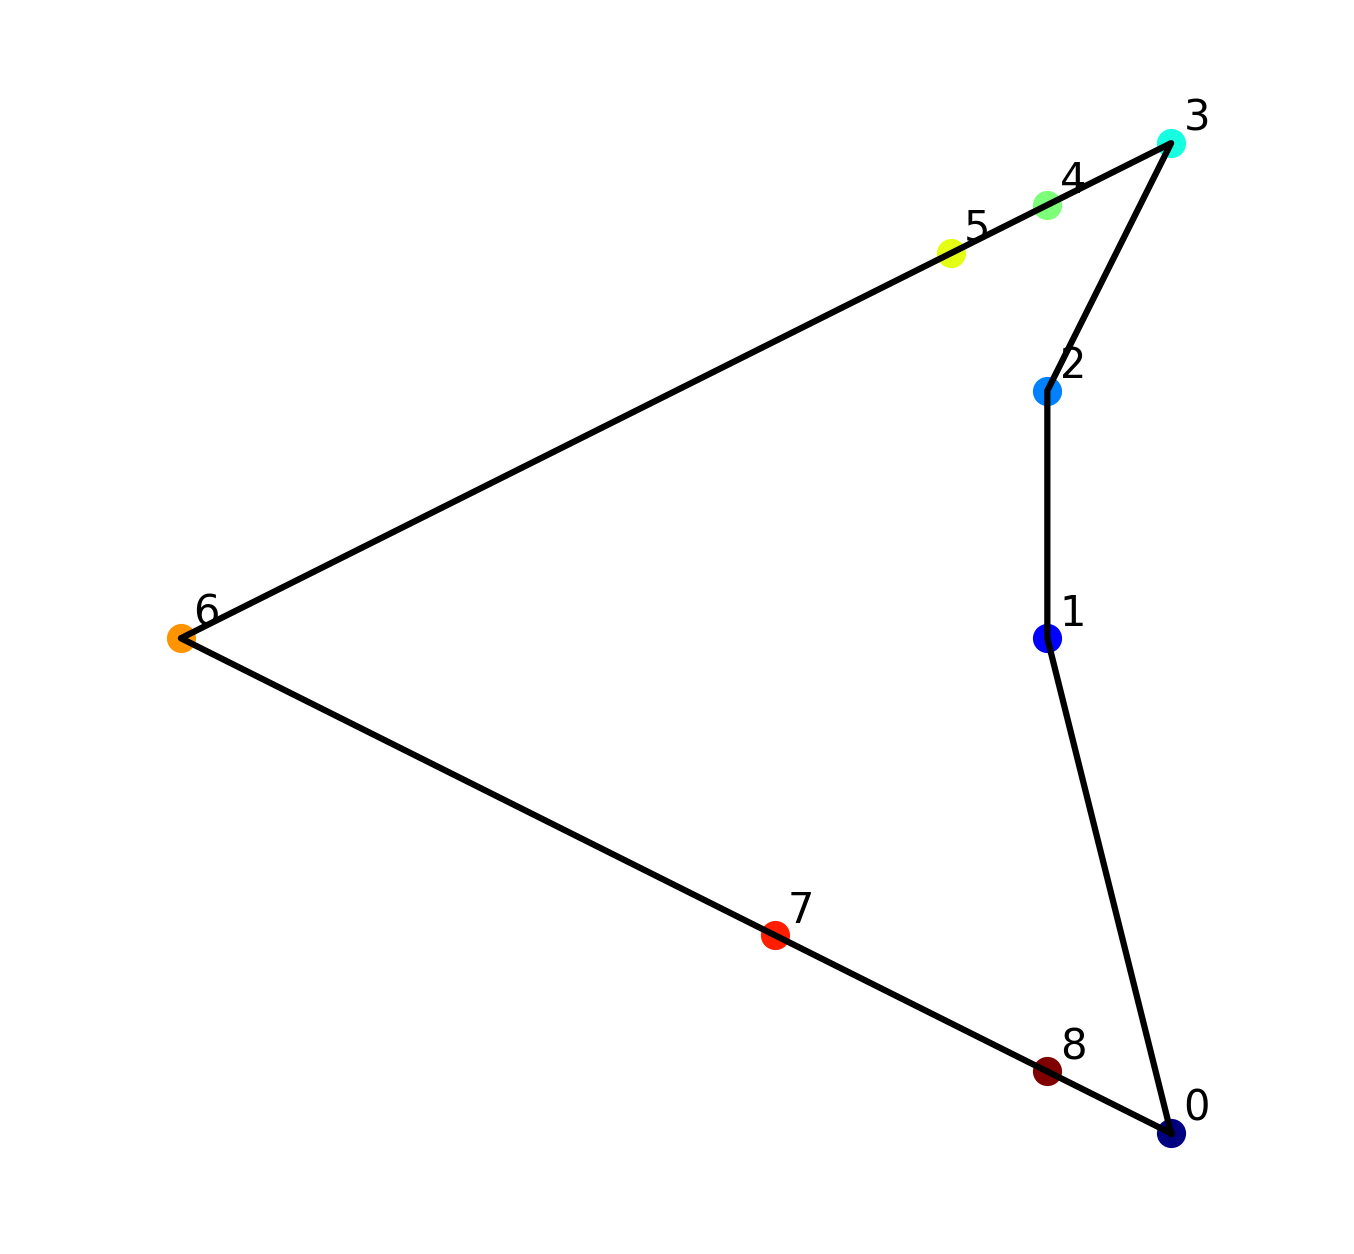
\includegraphics[width=0.7\linewidth]{figures/color_pent.png}
\captionof{figure}{\label{fig:color_pent}}
\end{subfigure}%
\begin{subfigure}{0.25\textwidth}
\centering
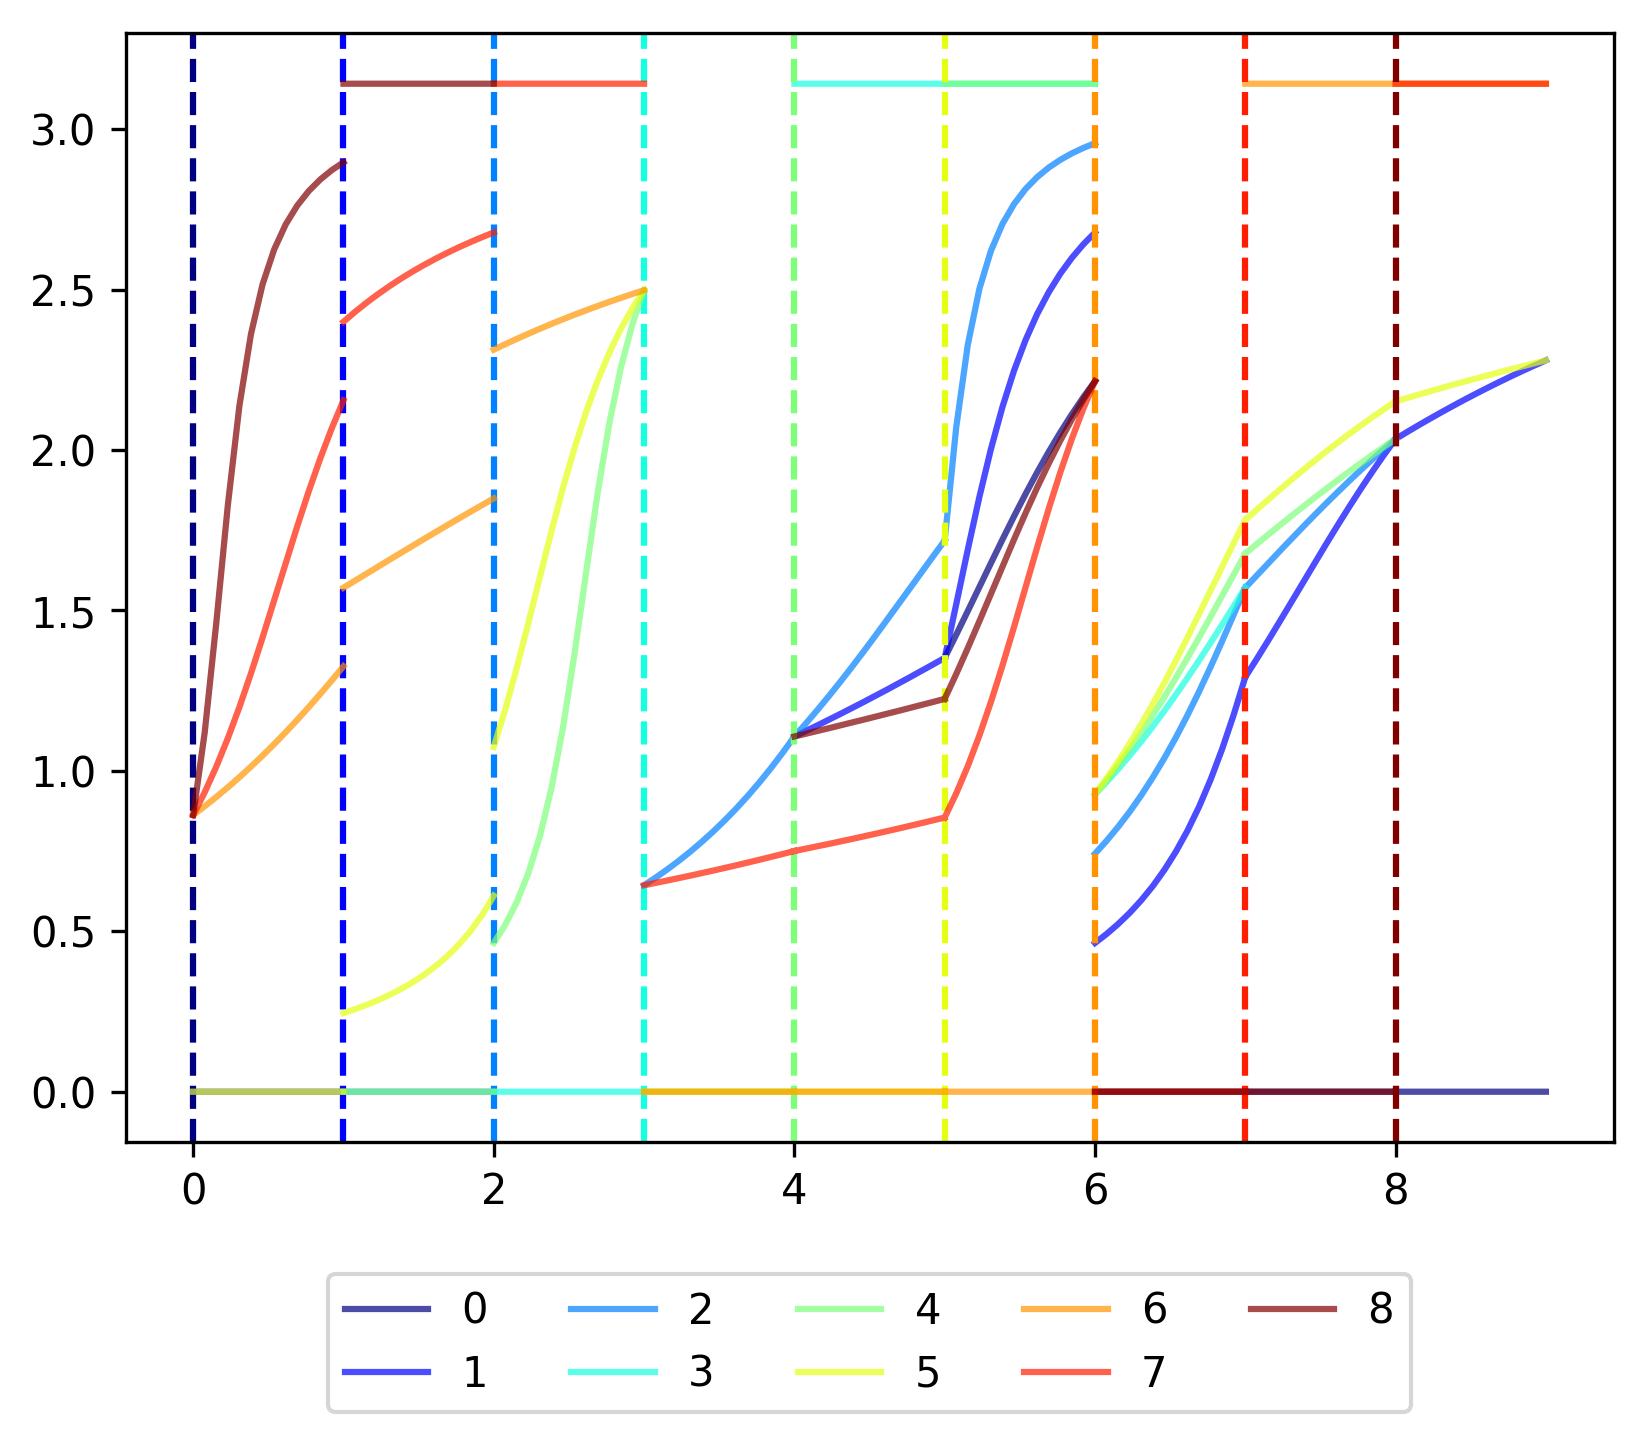
\includegraphics[width=0.8\linewidth]{figures/bvd.png}
\end{subfigure}
\caption{A polygon and its corresponding bounce visibility diagram.}
\label{fig:bvd}
\end{figure}


\subsection{Properties of BVD}
The bounce visibility diagram can generate the vertex visibility graph by construction. In \cite{rourke_viz}, the authors point out that if the robot can see a vertex, then it can see the two edges connected to that vertex if the vertex is convex; otherwise, it can see one of the edges connected to that vertex. As the robot moves along an edge in the original $P$, its vertex visibility view changes, as shown for $x\in (3, 6)$ in Fig~\ref{fig:bvd}. The region between curve 2 (blue) and curve 7 (red) is subdivided as the $x$ increases, which corresponds to the robot has increasing knowledge about things behind the gap between vertices $v_2$ and $v_7$ as it moves along the edge $v_3v_6$: the appearance of gap between vertices $v_1$ and $v_8$, and the appearance of vertex $v_0$. For $x\in (6, 9]$, the diagram shows a reverse process of disappearance of gaps. By incorporating the information of the appearance and disappearance of gaps, we can also generate the vertex-edge visibility graph from the bounce visibility diagram. 
% (\textcolor{red}{I don't have proof yet but I think there are enough info to do that. We can also shift this part about gap navigation into later sections.})

Circular symmetries in a polygon can be reflected in the periodic structure of the corresponding BVD, as shown in Fig~\ref{fig:regular_pent_bvd}.

\begin{figure}
% \makebox[\linewidth][c]{%
\begin{subfigure}{0.25\textwidth}
\centering
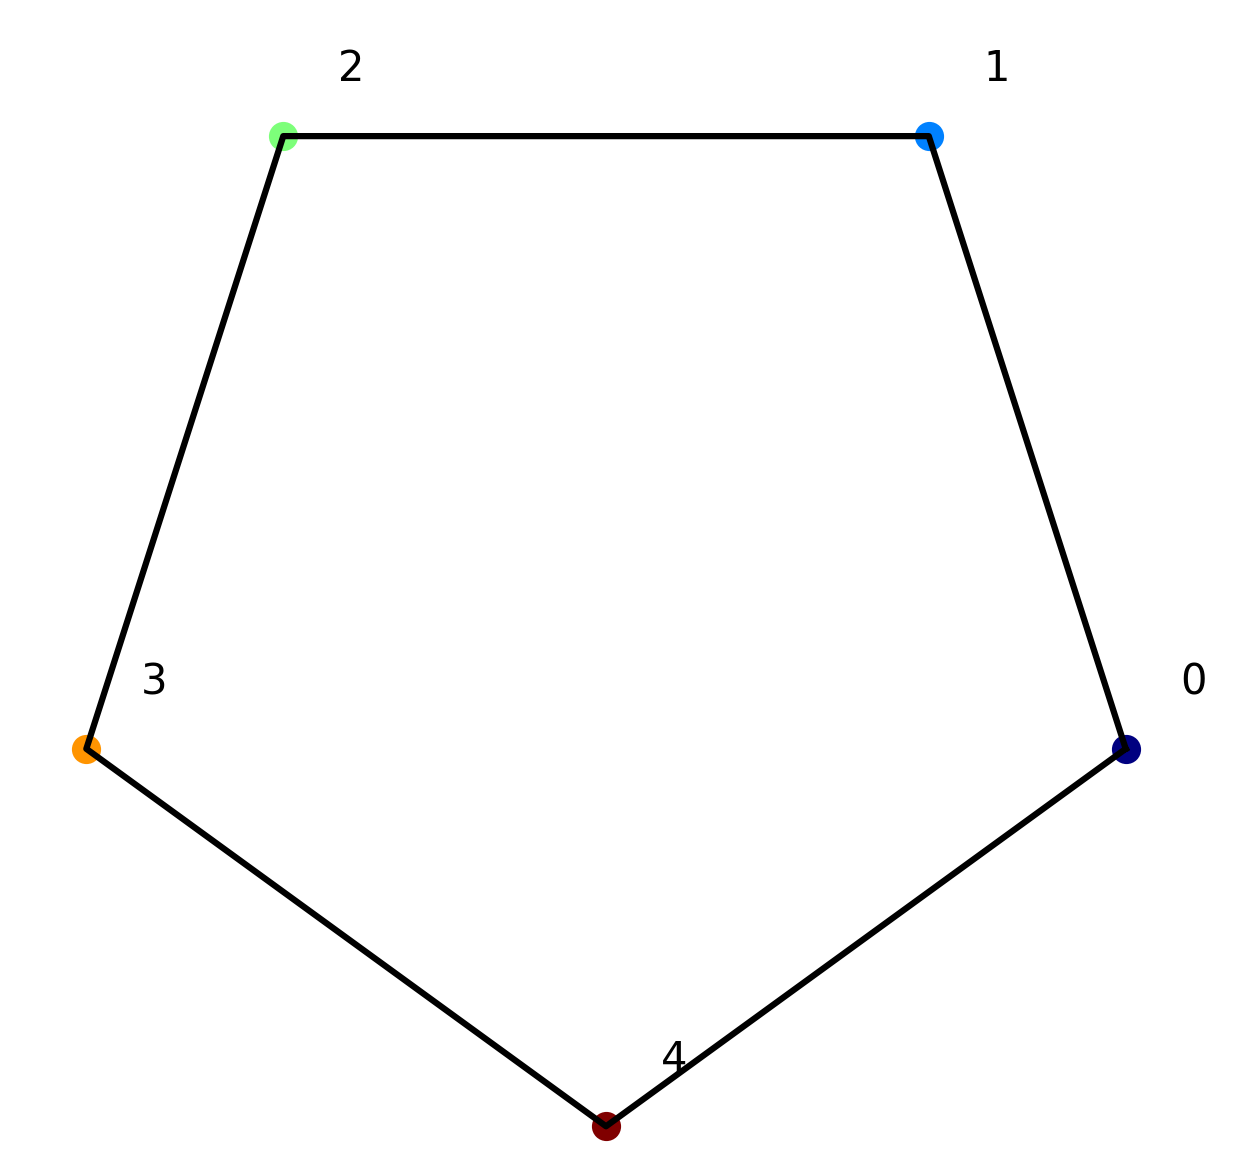
\includegraphics[width=0.5\linewidth]{figures/regular_pent.png}
\end{subfigure}%
\begin{subfigure}{0.25\textwidth}
\centering
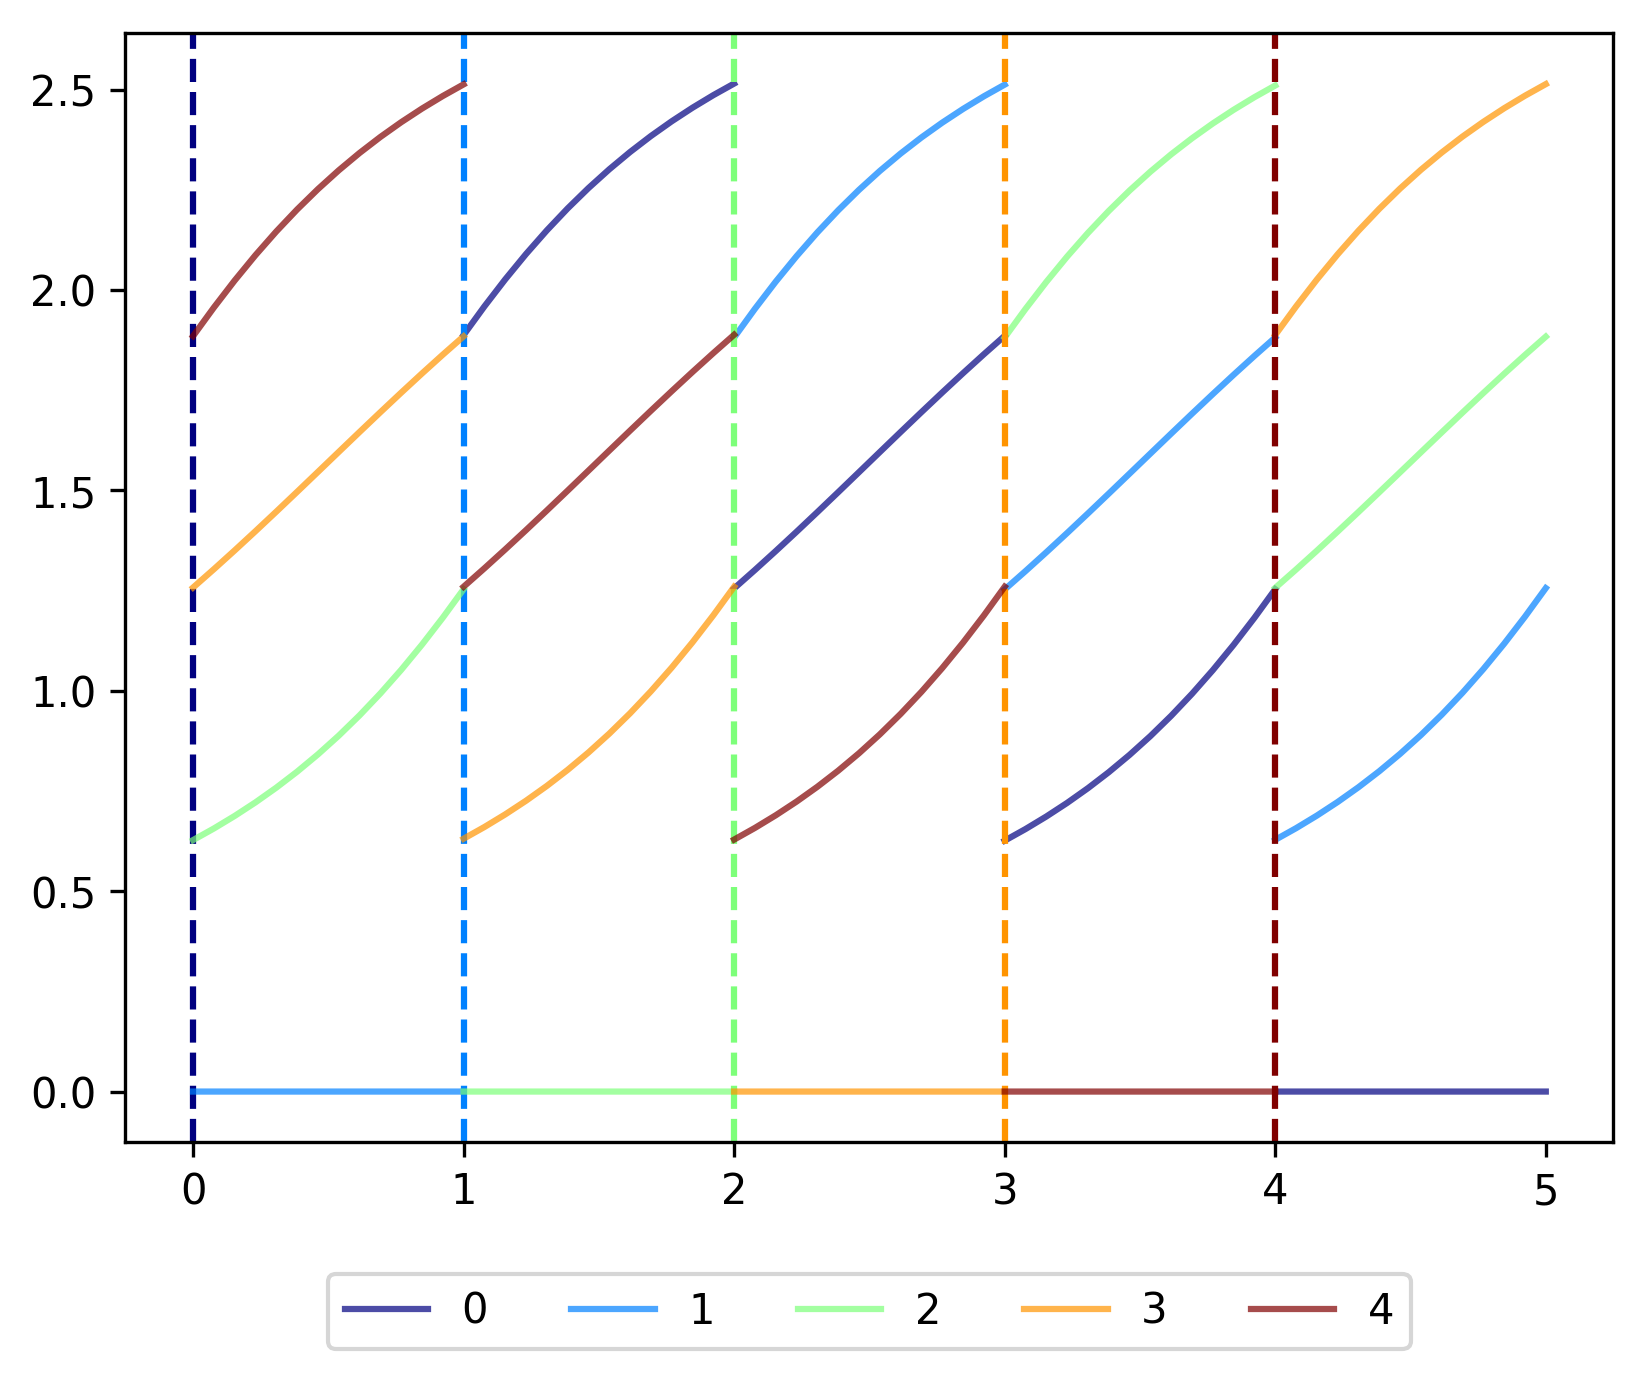
\includegraphics[width=0.8\linewidth]{figures/regular_pent_bvd.png}
\end{subfigure}
% }\\
\caption{The bounce visibility diagram for the regular pentagon. }
\label{fig:regular_pent_bvd}
\end{figure}



\begin{figure}
\centering
\makebox[\linewidth][c]{%

\begin{subfigure}{0.25\textwidth}
\centering
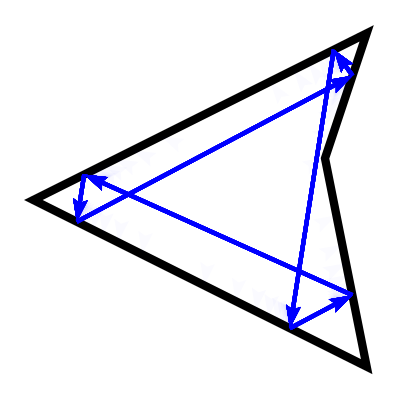
\includegraphics[width=0.45\linewidth]{figures/limit_cycle_concave_quad.png}
\captionof{figure}{\label{fig:limit_cycle}}
\end{subfigure}
\begin{subfigure}{0.25\textwidth}
\centering
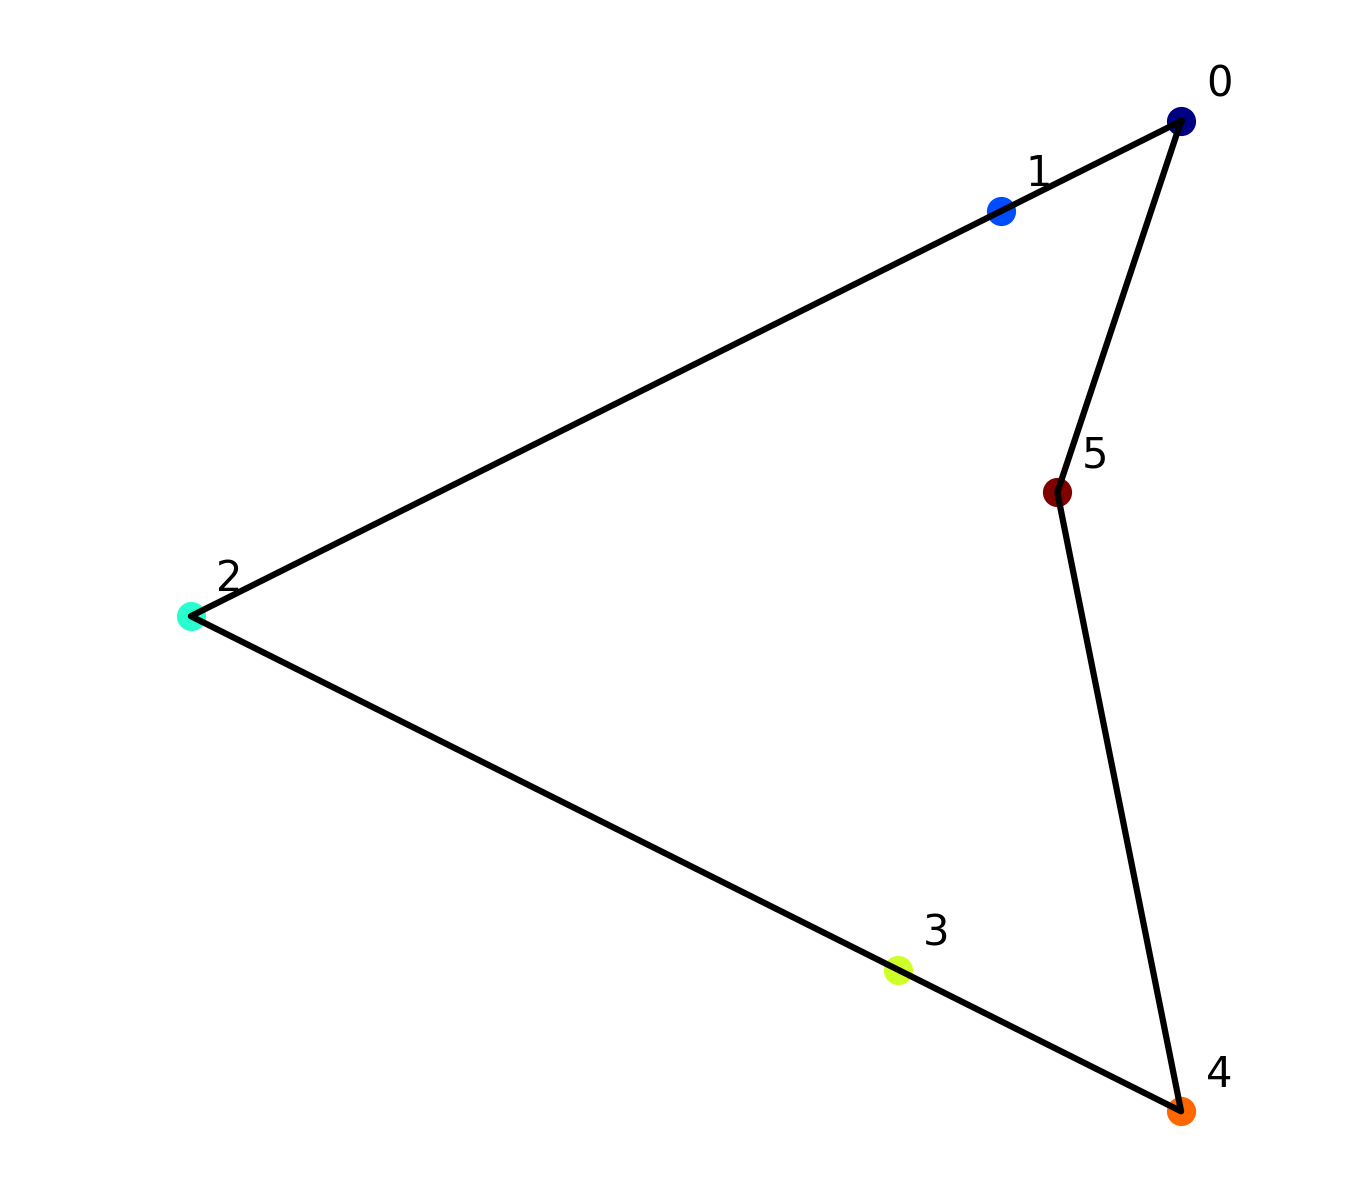
\includegraphics[width=0.52\linewidth]{figures/concave_quad.png}
\captionof{figure}{\label{fig:color_concave_quad}}
\end{subfigure}
}

\begin{subfigure}{0.25\textwidth}
\centering
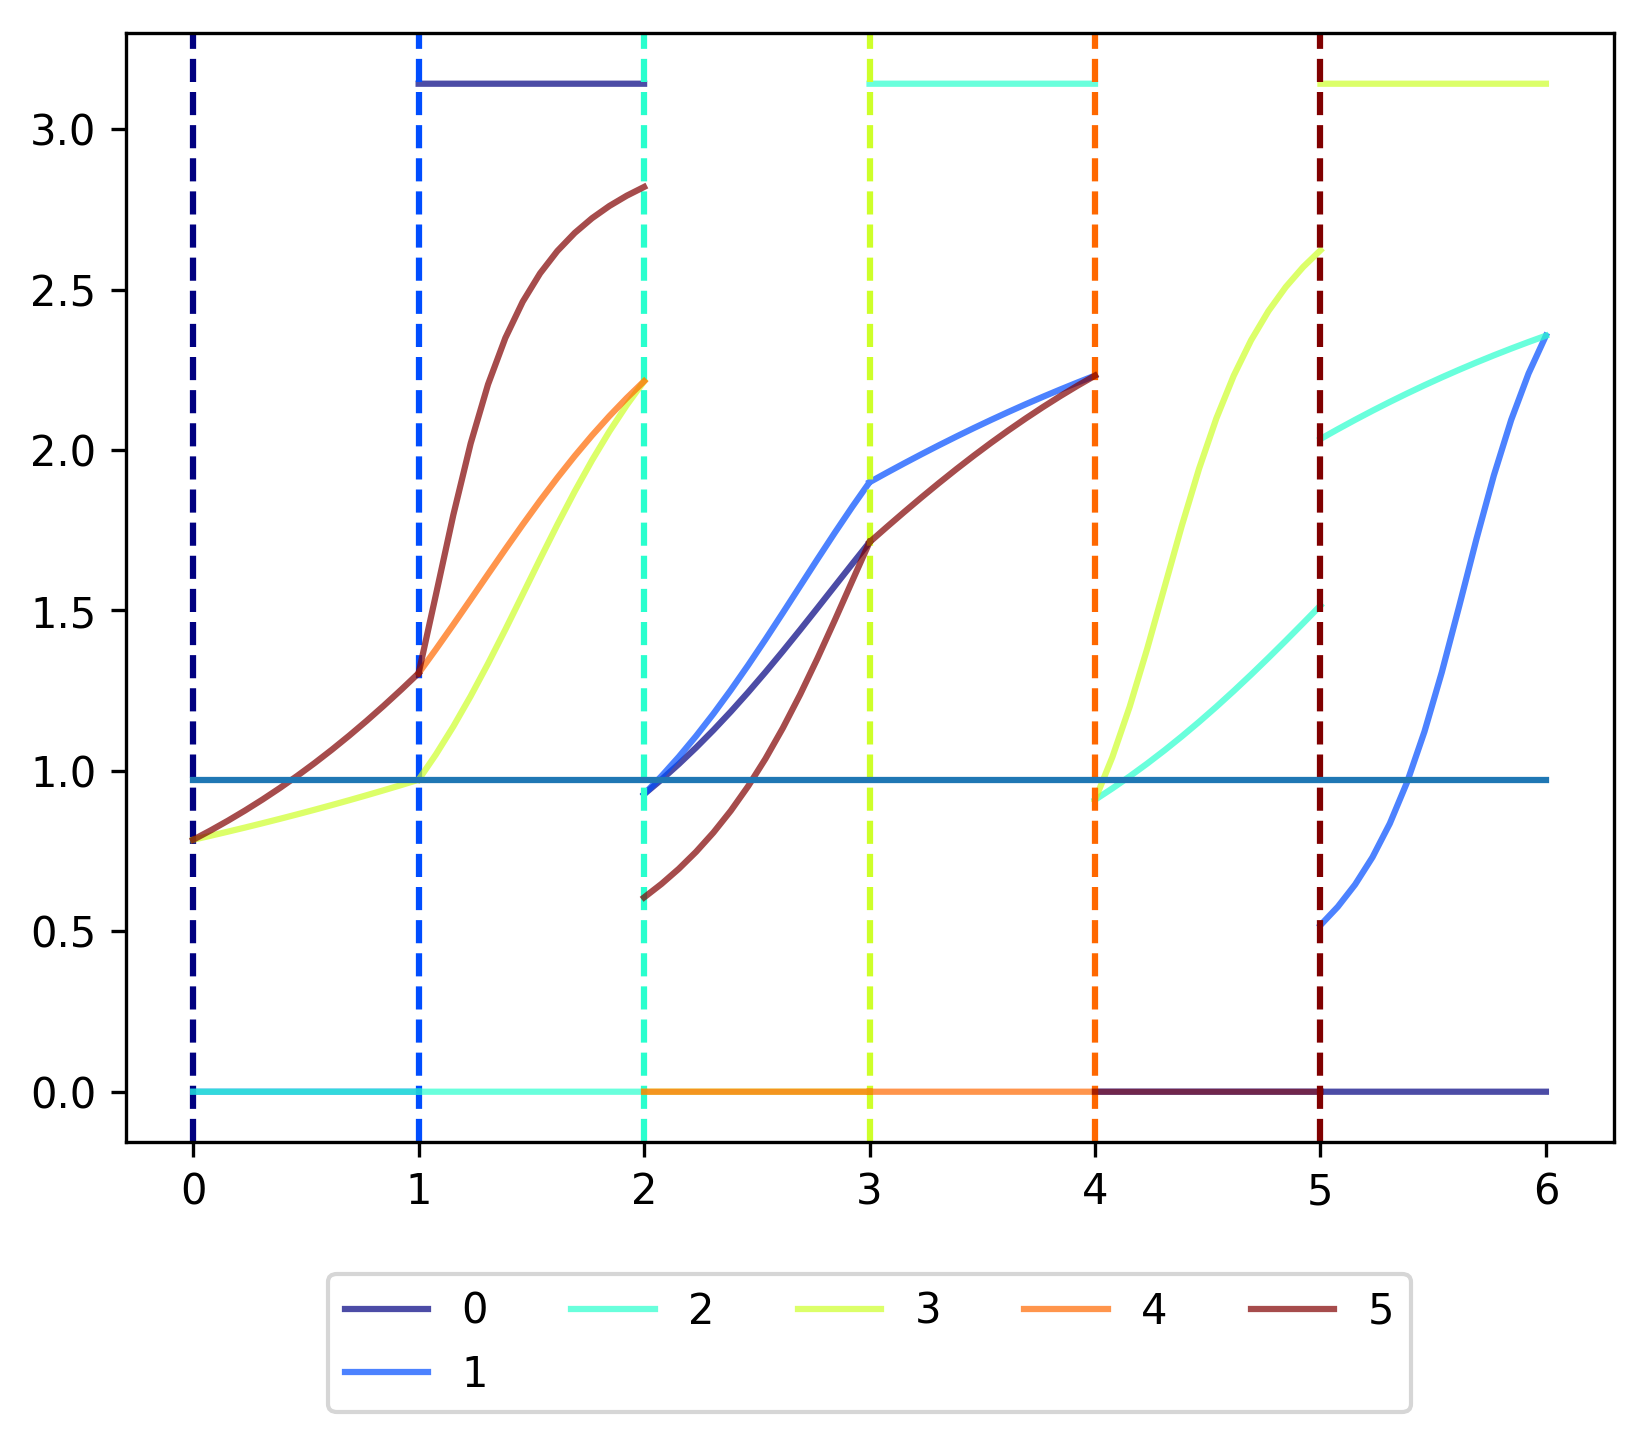
\includegraphics[width=0.8\linewidth]{figures/limit_cycle_bvd.png}
\captionof{figure}{\label{fig:concave_quad_bvd}}
\end{subfigure}%
\begin{subfigure}{0.25\textwidth}
\centering
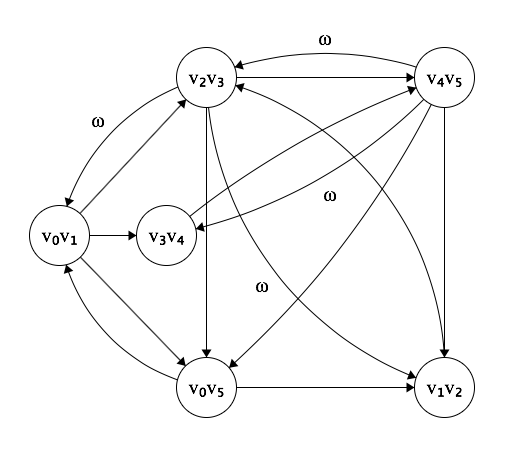
\includegraphics[width=0.8\linewidth]{figures/limit_cycle_graph.png}
\captionof{figure}{\label{fig:limit_cycle_diagram}}
\end{subfigure}
\caption{The bounce visibility diagram with limit cycle information}
\label{fig:limit_cycle_bvd}
\end{figure}

\subsection{Combinatorial Complexity of BVD}

To consider the size of the bounce visibility diagram for an input polygon $P$ with $n$ vertices, we let $r$ be the number of reflex vertices in the polygon, and $m$ be the average number of visible vertices to a vertex in $P'$. For a convex vertex, its partial local sequence will not have new vertex that is not in $P$, while for a reflex vertex, we can have $O(n)$ new vertices. We can have as many as half of the vertices to be reflex, so $r = O(n)$; each of the reflex vertices can produce $O(n)$ new vertices in its partial local sequence, so the size of $P'$ is $O(n^2)$. It is possible for a vertex in $P'$ to see all other vertex, so, in the worse case, $m = O(n^2)$. Therefore, the complexity of the bounce visibility diagram is $O(n\cdot r\cdot m) = O(n^4)$. 

We might hope that if $r$ is large, then not all of the reflex vertices will produce a large number of new vertices, or that if there are many new vertices, then the new vertices will not have good visibility in $P'$ since most of them will be inserted into a corner of the polygon, and then we can bound the complexity of the BVD. Unfortunately, the number of reflex vertices, the new vertices produced in their partial local sequence, and the new vertices' visibility can be large at the same time. We will present a family of input polygons with BVD of $\Theta(n^4)$ complexity as follows. 

\begin{figure}
%\hspace{-40px}
\centering
%\makebox[\linewidth][c]{%
%\hspace{30px}
\begin{subfigure}{0.25\textwidth}
\centering
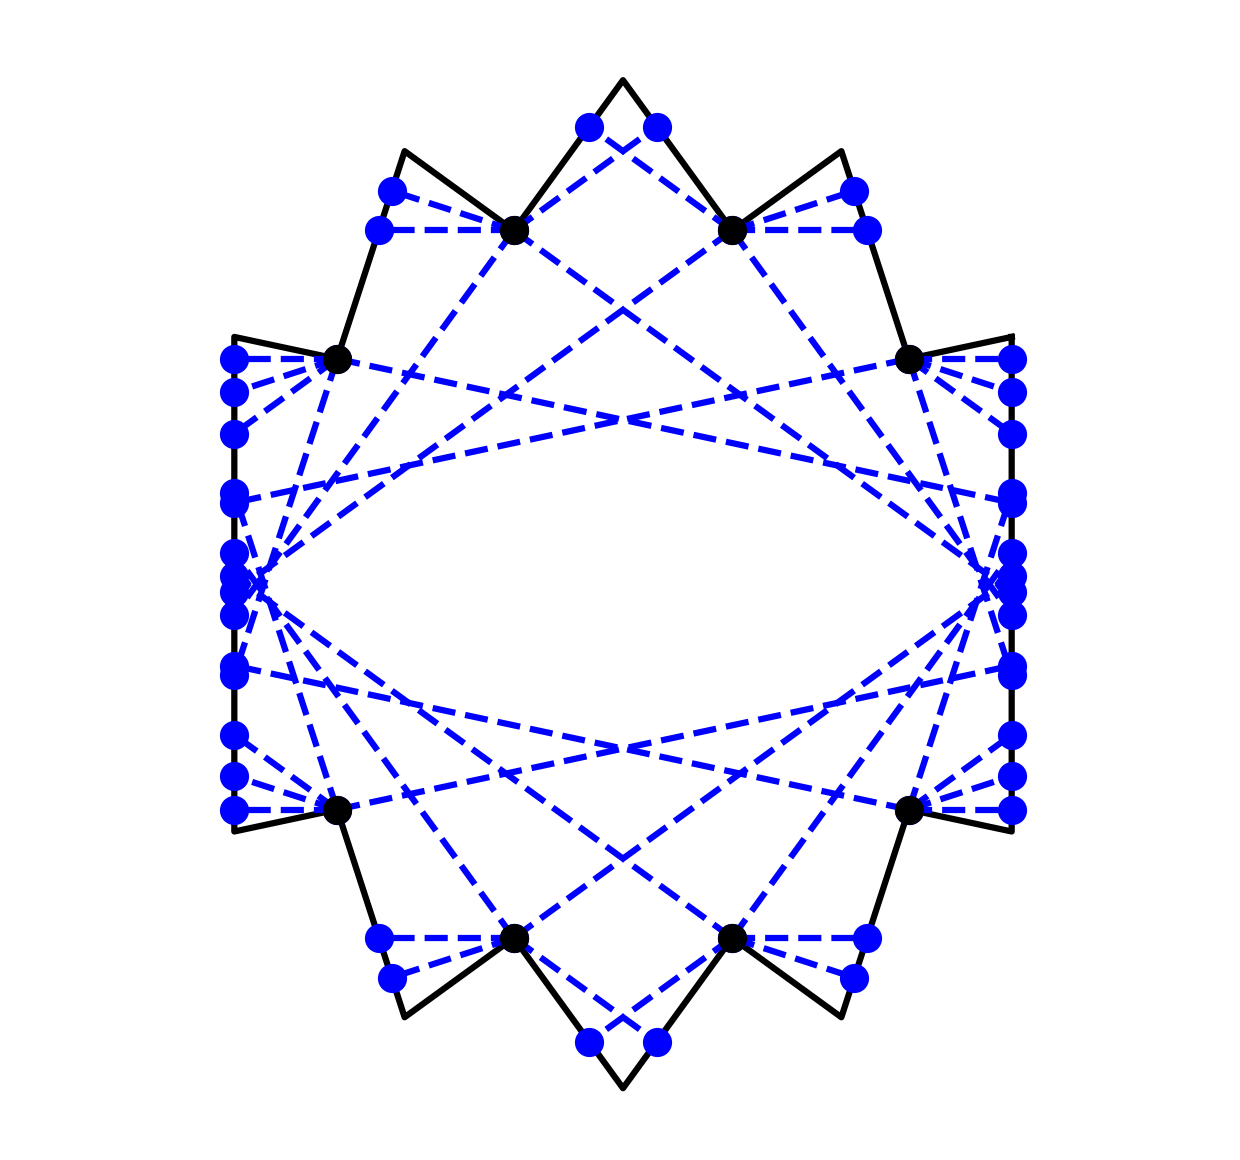
\includegraphics[width=0.7\linewidth]{figures/chestnut_5.png}
\label{fig:t4}
\end{subfigure}
%\hspace{-40px}

\begin{subfigure}{0.25\textwidth}
\centering
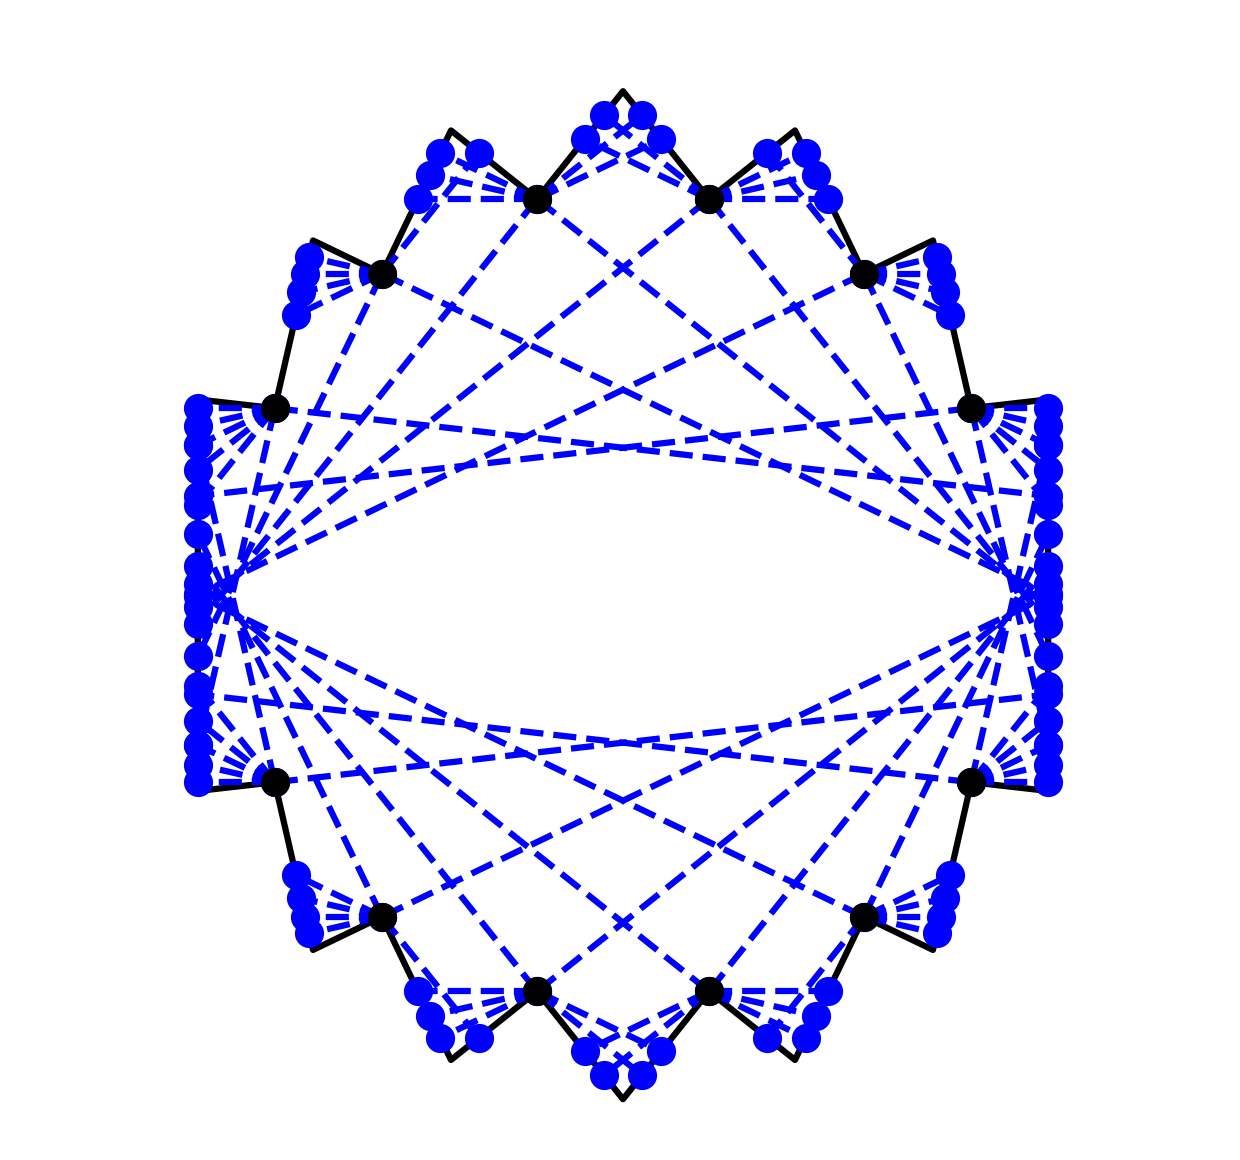
\includegraphics[width=0.7\linewidth]{figures/chestnut_7.png}
\label{fig:t6}
\end{subfigure}\\
\caption{The worse case polygon for $t = 4$ and $t = 6$ 
\label{fig:chestnut}}
\end{figure}

Let $n = 4t+2$, where $t$ is a positive integer. We design a polygon with
$r = 2t$ reflex vertices. The polygon is symmetric with respect to its medium
horizontal line. In the top half, the reflex vertices are uniformly located on a
circle and thus they are visible to each other; the convex vertices are chosen
so that they are outside the circle and the line through an edge will not
intersect other edges. Each reflex vertices will have at least $t-1$ new
vertices in its partial local sequence. All vertices in the top half can see
each vertex in the bottom half and vice versa. So there will be $2t(t-1)+n$
vertices in the polygon after we insert all new vertices in the partial local
sequence for all reflex vertices. Each of them can see at least $t(t-1)+n/2$
other vertices. The final complexity for the bounce visibility diagram is
$\Theta ((2t(t-1)+n)(t(t-1)+n/2)) = \Theta (t^4) = \Theta(n^4)$.
Fig \ref{fig:chestnut} shows the polygons for $t = 4$ and $t=6$ with all the
vertices in the partial local sequences. % show the diagram to edge

% show the fix bounce
% show the periodic behavior
% show the gap navigation
% show we could find equivalent class on theta
% \begin{itemize}
% \item Big O complexity of construction, and size of resulting graph


\section{BVD as an Information Space \label{bvd_info}}

Information spaces \cite{tovar2005information} are a useful formalism for
reasoning about the information available to a robot as a result of its sensor
and action history. From the \emph{history information space} (the space of all
sensor/action histories), we can define mappings to other, more useful spaces.

Here we will show that the bounce visibility diagram can induce a useful
information space for many mobile robot tasks, and can be augmented with
information from the geometric properties of actuators and sensors.

We will construct $G_{BVD}$, a graph where nodes are segments in the decomposed
environment $P'$ constructed in Section \ref{bvd_def}.

We then define edges in this graph to be transitions between these segments, based on the bounce laws and
required to transition between them. First, we observe that any two segments in
$P'$ that are visible at all are visible along their entire lengths. Thus, we
there exists a function $f$ which maps a point $s \in v_i
v_{i+1}$ to a point $f(s) \in v_j v_{j+1}$ under a bounce at angle $\theta$ from
the normal on edge $v_i v_{i+1}$, for all valid ranges of $s$, $f(s)$, and
$\theta$.

Rather than use $f$ directly, we take a nondeterministic approach and define a
directed transition between edges $v_i v_{i+1}$ and $v_j v_{j+1}$ if it is
possible to reach edge $v_j v_{j+1}$ from edge $v_i v_{i+1}$ under any bounce.
We label the edge with the range of bounce angles, $\theta_{min} < \theta <
\theta_{max}$, under which this is possible. See Figure \ref{fig:bounce_range} for
the geometric definitions of $\theta_{max}$ and $\theta_{min}$.

\begin{figure}
    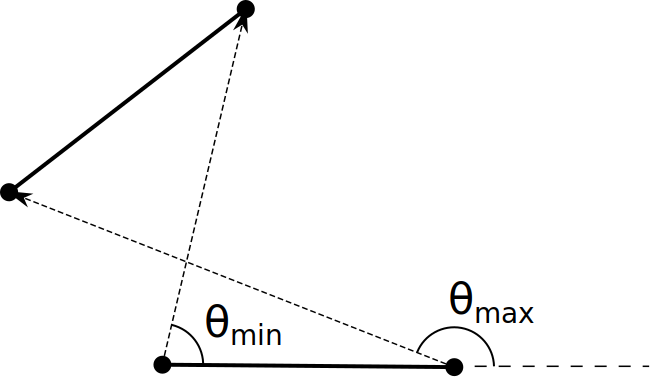
\includegraphics[width=0.8\linewidth]{figures/bouncerange.png}
    \centering
    \caption{Definitions of $\theta_{max}$ and $\theta_{min}$. Can be computed
by rotating the source edge to the x axis without loss of generality.}\label{fig:bounce_range}
    \centering
\end{figure}

\subsection{Augmenting the Graph with Dynamical Information}

We can also add information to the edges in $G_{BVD}$ indicating whether the
mapping from one edge to another is a \emph{contraction mapping}: a transition
which will bring two separate points in the domain closer together in the range,
a useful property for reducing state uncertainty and engineering limit cycles,
as will be discussed in Section \ref{patrol}.

The necessary condition for $f$ to be a contraction mapping is:

\begin{equation*}
|f(x) - f(y)| \leq c |x-y|
\end{equation*}

such that $0 \leq c < 1$.

From Figure \ref{fig:cont_map}, we can see that

\begin{equation*}
|f(x) - f(y)| = \frac{\sin(\theta - \phi)}{\sin(\pi-\theta)} |x-y|
\end{equation*}

from the law of sines, where $\phi$ is the angle between the two edges if they
are extended to their intersection point. If the edges are parallel, a
contraction map is not possible (points will maintain their distance, not shrink
closer together). Thus, whenever $\frac{\sin(\theta - \phi)}{\sin(\pi-\theta)}
< 1$, $f$ is a contraction map, and the edge from $v_i v_{i+1}$ to $v_j
v_{j+1}$ can be labelled as such, with the range of $\theta$ which makes this
condition true.

Furthermore, the contraction property of a composition of multiple bounces can
be determined by simply multiplying the coefficients $\frac{\sin(\theta_i -
\phi_i)}{\sin(\pi-\theta_i)}$, and the constraints on the satisfying angles
$\theta_i$ can be propagated through the composition.

\begin{figure}
    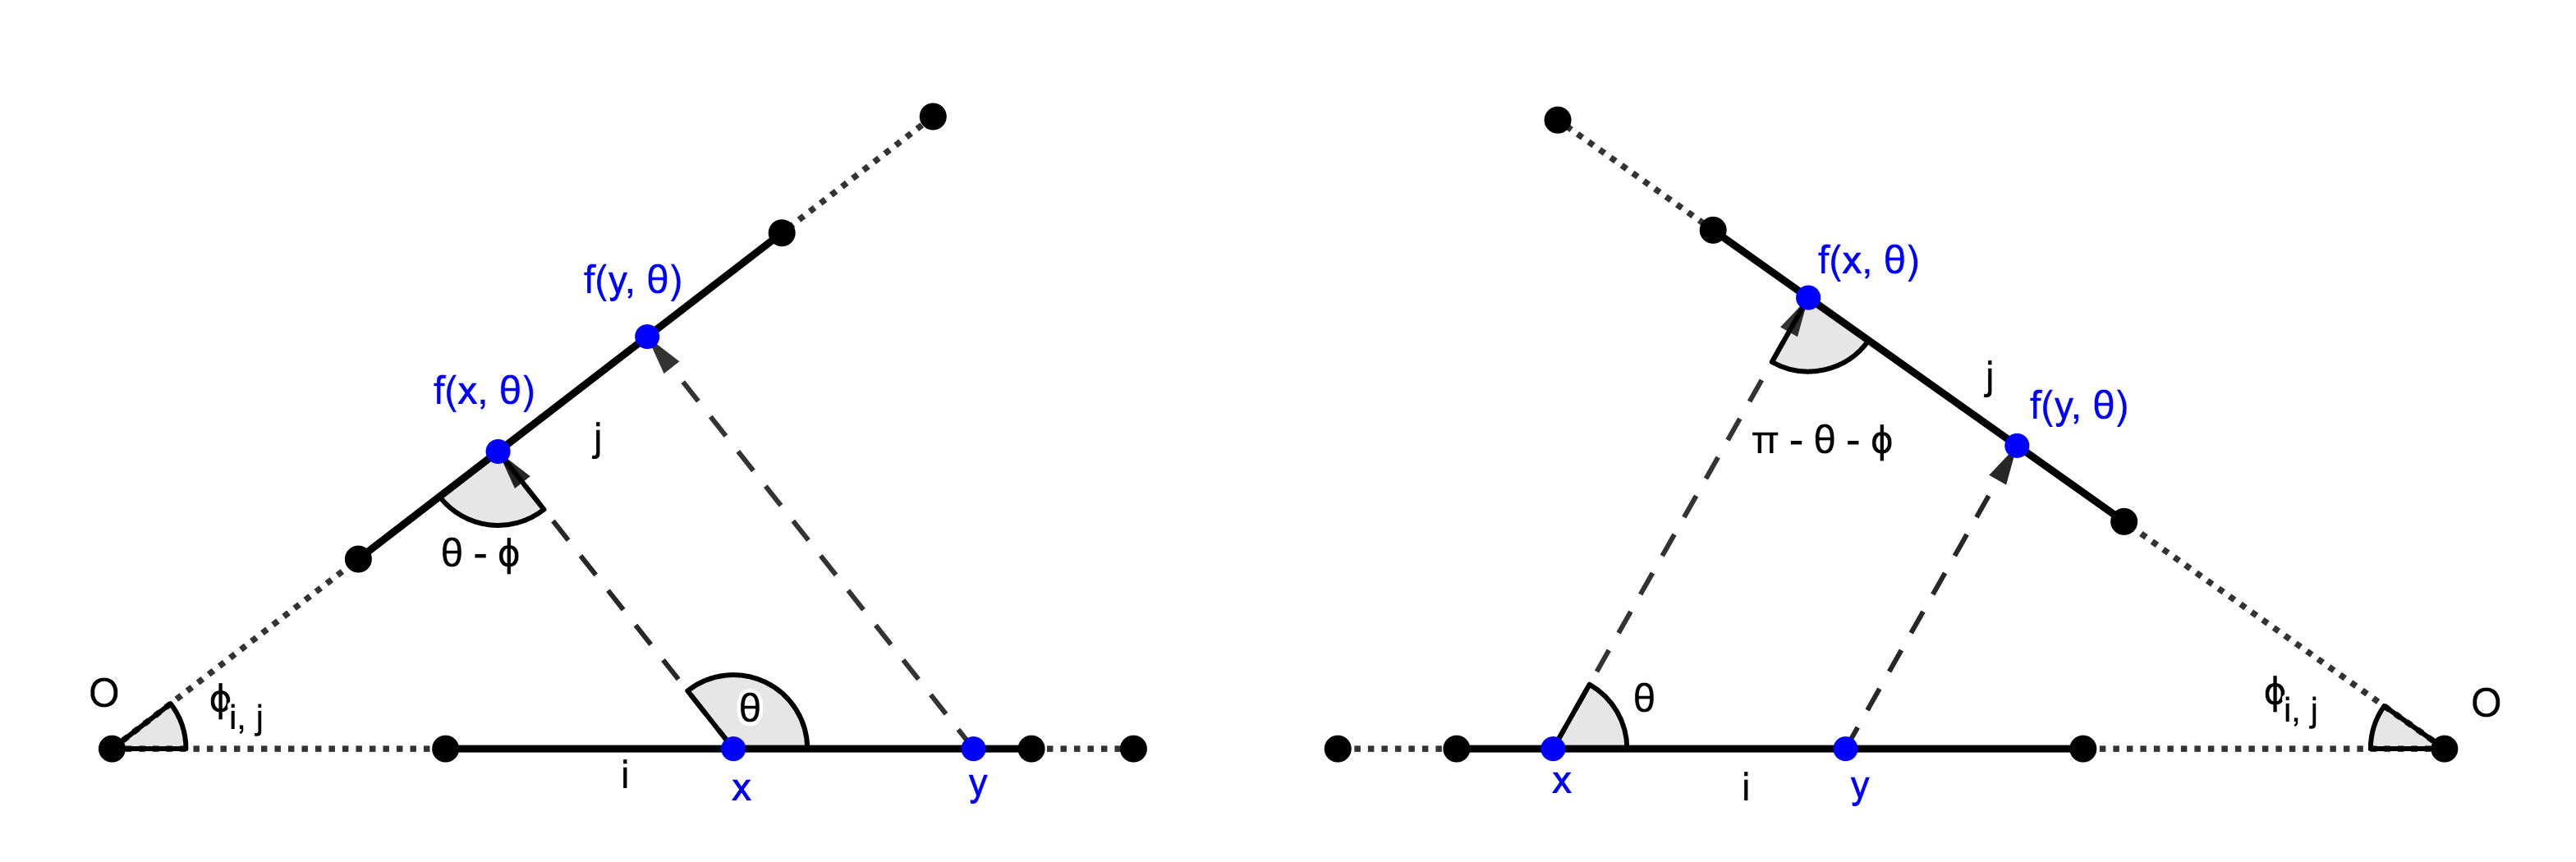
\includegraphics[width=0.8\linewidth]{figures/contraction_map_cond.png}
    \centering
    \caption{\label{fig:cont_map}}
    \centering
\end{figure}

\subsection{Sensor Modelling}

Here we sketch how different virtual sensors may be incorporated into this
information space representation.

\begin{itemize}
\item \emph{Laser Beams:} laser beams form new, internal edges of the polygon. They can be
added to the bounce visibility graph by marking all the edges which represent
bounces that would cross the laser beam with a special symbol. different symbols
for distinguishable beams. If a beam is encountered, and we are tracking state
as a set of possible segments along the boundary of $P'$, we can reduce
uncertainty in our estimate by only propagating the state estimate
forward along edges with that symbol. To engineer reduction in uncertainty,
we may be able to put laser beams in positions that break graph symmetry.
\item \emph{Pebbles:} pebbles are quite important in many robotic tasks, such as
when we need to guarantee that a wall-following strategy has successfully
circumnavigated a polygon. In this representation, we can simply augment nodes
in $G_{BVE}$ if our robot has placed a pebble in that segment (or we may mark
multiple nodes, then use actions to reduce uncertainty in our state estimate
once we return to the pebble).
\item \emph{Cameras:} Especially when discussing coverage, it is helpful to have
some sense of how we "cover" a polygon's interior. One abstract sensor with this
behavior is a model of a camera, which may have some given range and field of
view. The set-theoretic representation of this visibility region can be used to
represent how much of the polygon may be covered by a given trajectory. Ideally,
coverage strategies would allow for satisfying coverage given nondeterminism in
the start states and actions.
\end{itemize}

\section{Task Formulation}

We will now show how to formulate many common robot task specifications in terms
of the data structure described above. The discretization of the continuous
environment allows us to now reason over trajectories through a graph.


\subsection{Navigation}

Here, we define the \emph{navigation} task as:

\begin{quotation}
Given an environment $P$, a start set of possible robot positions along the
environment boundary $S$, and a goal set $G$, determine a strategy $\pi$ which
will be guaranteed to take the robot from any point in $S$ to a point in $G$.
\end{quotation}

If the start set $S$ is such that it is equal to one of the equivalence
classes of the data structure, a navigation query is simple - the start set in
the graph is a single node, and the query is solved by a shortest path from this
node to the nodes representing the goal set. The shortest path will correspond
to the navigation strategy with the fewest number of bounces. It would also be
possible to determine the shortest path in the metric space of the polygonal
environment, either by adding weights to the edges in the graph, or by
leveraging results from shortest path navigation using visibility diagrams.

It may be
interesting to instead look to solve the navigation problem with different
criteria than the smallest number of bounces - for instance, we may look for a
strategy which uses the fewest number of bounce angles, or has the fewest number
of switches between bounce angles (especially useful for a robot which changes
its bounce angle mechanically).

If the start set $S$ lies in more than node of the graph, things get a bit
trickier. We need to guarantee all-path reachability for a set of start nodes in
a graph. There are also complications if the user-specified start set does not
exactly overlap the equivalence classes formed by the decomposition in Section
\ref{bvd_def}. For now, we can only guarantee navigation from one equivalence
class (segment along the new polygon $P'$) to another.



\subsection{Patrolling \label{patrol}}

We define the \emph{patrolling} task as:

\begin{quotation}
Given an environment $P$, a set of possible starting states $S$, and
a sequence of edges of the environment $E = \{e_1, \ldots, e_k\}$,
determine a strategy which causes the robot to visit each edge of the sequence
in order on a repeatable path.
\end{quotation}

This task is related to the Aquarium Keeper's Problem in computational
geometry \cite{czyzowicz1991aquarium}.

In prior work \cite{NilBecLav17}, it was shown that stable limit cycles
exist for constant-angle fixed bouncing in regular polygons, for some ranges of bounce angles.
These results also hold for convex polygons in general.

The general flavor of these results are that the bounce functions from edge to
edge are composed into one function which returns the robot to its starting
edge. If this function is a contraction map, a fixed point exists on the
starting edge, and thus a limit cycle of the robot's trajectory exists. The
exact conditions of the existence of this limit cycle depend on the product of
the contraction coefficients being less than one; and on $\theta$ being such
that the bounce at each stage can actually occur. All of the information
necessary to check these conditions is in $G_{BVD}$, as described in Section
\ref{bvd_info}.

Thus, finding all possible limit cycles in an environment $P$ amounts to finding
all cycles in $G_{BVD}$ such that this condition holds.

To examine the behavior of a robot with a given fixed bounce angle, such as the
analysis in \cite{ErLav13}, we can easily extract information for the fixed angle bouncing strategy
mentioned in section \ref{subsec:bounce_strategy} by overlaying an horizontal
line $\theta = \theta_0$ onto the BVD, where $\theta_0$ is the angle chosen by
the bouncing strategy. In Fig \ref{fig:limit_cycle_bvd}, one of the possible
limit cycle with fixed angle $\theta = 0.6$ for the concave quadrilateral is
shown in Fig \ref{fig:limit_cycle}; the bounce visibility diagram for this
polygon is shown in Fig \ref{fig:concave_quad_bvd} with the horizontal line
$\theta = \theta_0$, where $\theta_0 = \frac{\pi}{2}-0.6$ (we need to convert
the angle from w.r.t the normal of the wall to w.r.t the forward direction of
the robot). The horizontal line cut through different regions of the diagram,
representing the possible edges that the robot can bounce to at different points
on the boundary with bounce angle $\theta_0$. For example, at edge $v_5v_0$, the
robot can bounce to edge $v_0v_1$ and $v_1v_2$. We can create a graph for
$\theta = \theta_0$, whose nodes are edges in $P'$ and two nodes are connected
by a directed edge if the robot can bounce from one edge to another at
$\theta_0$, as shown in Fig \ref{fig:limit_cycle_diagram}. It is more stable
for the robot to bounce to some edges than others. In the diagram
(Fig \ref{fig:concave_quad_bvd}), the line $\theta = \theta_0$ cuts through
four different regions for $x \in (2, 3)$, but the sections for $v_4v_5$ and
$v_0v_5$ are much larger than those for $v_0v_1$ and $v_1v_2$. So we know it is
more likely and more stable for the robot to bounce to edge $v_4v_5$ and
$v_0v_5$. We marked the edge with unstable bounce in the graph with $\omega$ in
Fig \ref{fig:limit_cycle_diagram}. The limit cycle shown in
Fig \ref{fig:limit_cycle} corresponds to the cycle
$v_0v_1\rightarrow v_3v_4\rightarrow v_4v_5 \rightarrow v_1v_2 \rightarrow v_2v_3 \rightarrow v_0v_5 \rightarrow v_0v_1$
in Fig \ref{fig:limit_cycle_diagram}.

\subsection{Localization}

We define the \emph{localization} task as:

\begin{quotation}
Given an accurate map of the environment, but no knowledge of configuration,
determine a strategy which eliminates uncertainty in configuration as much as
possible (ideally, to a point in configuration space).
\end{quotation}

In \cite{OkaLav06}, the authors show that localization is possible with
mobile robots with a linear and angular odometer, or a compass and contact
sensor, but not with robots with only an angular odometer and contact sensor.
These sensing configurations correspond to which types of bounce laws each robot
is capable of performing, and we would like to be able to rederive the same
results in this representation.

Localization amounts to a path finding algorithm in the larger graph, where each
node is an element of the powerset of segments along $P'$. Future work will
include how to tractibly search this graph (such as heuristics for doing so
which take advantage of the uncertainty-reducing properties of contraction
mappings).


\section{Open Questions and Future Work}

Future work also includes:

\begin{itemize}
\item Characterizing the completeness and correctness of algorithms for
navigation, coverage, localization, etc.
\item Continue to place this work in context, especially with BitBots, Gap
Navigation Trees, and Combinatorial Visibility Vectors
\item Developing ways to query two $G_{BVD}$s, generated with different constraints on
 bouncing laws and sensors, and determine whether one represents a robot which
is ``more powerful" than another. Perhaps this will require a clever
parameterization of bouncing laws.
\item Investigate how to generate bounce law distributions that allow a bounce
to be randomly selected at each stage and guarantee some properties about the
resulting trajectory
\item Extending analysis to more tasks, such as coverage and pursuit-evasion
\end{itemize}



\bibliographystyle{IEEEtran}
\bibliography{/home/alli/common/refs}

\end{document}
